\documentclass[final]{fhnwreport}         %[mode] = draft or final
%%---Main Packages-----------------------------------------------------------------------
\usepackage[english, ngerman]{babel}	%Mul­tilin­gual sup­port for LaTeX
\usepackage[T1]{fontenc}				      %Stan­dard pack­age for se­lect­ing font en­cod­ings
\usepackage[utf8]{inputenc}				  %Ac­cept dif­fer­ent in­put en­cod­ings
\usepackage{lmodern}                 %The newer Font-Set
\usepackage{textcomp}					      %LaTeX sup­port for the Text Com­pan­ion fonts
\usepackage{graphicx} 					      %En­hanced sup­port for graph­ics
\usepackage{float}						        %Im­proved in­ter­face for float­ing ob­jects
%\usepackage{ifdraft}                %Let you check if the doc is in draft mode

%%---Useful Packages---------------------------------------------------------------------
%\usepackage[pdftex,dvipsnames,tables]{xcolor}  %Driver-in­de­pen­dent color ex­ten­sions for LaTeX
\usepackage[table,xcdraw]{xcolor}
\usepackage{csquotes}                %Simpler quoting with \enquote{}
\usepackage{siunitx} 					      %A com­pre­hen­sive (SI) units pack­age
\usepackage{listings}					      %Type­set source code list­ings us­ing LaTeX
\usepackage[bottom]{footmisc}			  %A range of foot­note op­tions
\usepackage{footnote}					      %Im­prove on LaTeX's foot­note han­dling
\usepackage{verbatim}					      %Reim­ple­men­ta­tion of and ex­ten­sions to LaTeX ver­ba­tim
\usepackage[textsize=footnotesize]{todonotes} %Mark­ing things to do in a LaTeX doc­u­ment
\usepackage{lipsum}              % Gives you access to blindtext

%%---Tikz Packages-----------------------------------------------------------------------
%\usepackage{standalone}
%\usepackage{tikz}
%\usepackage{circuitikz}
%\usetikzlibrary{arrows}
%\usetikzlibrary{calc}
%\usetikzlibrary{intersections}

%%---Math Packages-----------------------------------------------------------------------
\usepackage{amsmath}					    %AMS math­e­mat­i­cal fa­cil­i­ties for LaTeX
%\usepackage{amssymb}					  %Type­set­ting symbols (AMS style)
%\usepackage{array}						  %Ex­tend­ing the ar­ray and tab­u­lar en­vi­ron­ments
%\usepackage{amsthm}					    %Type­set­ting the­o­rems (AMS style)

%%---Table Packages----------------------------------------------------------------------
\usepackage{tabularx}					  %Tab­u­lars with ad­justable-width columns
%\usepackage{longtable}
\usepackage{multirow}					  %Create tab­u­lar cells span­ning mul­ti­ple rows
\usepackage{multicol}					  %In­ter­mix sin­gle and mul­ti­ple columns
\usepackage{graphicx}
\usepackage{colortbl}

%%---PDF / Figure Packages---------------------------------------------------------------
\usepackage{pdfpages}					  %In­clude PDF doc­u­ments in LaTeX
\usepackage{pdflscape}					  %Make land­scape pages dis­play as land­scape
%\usepackage{subfig}					    %Fig­ures di­vided into sub­fig­ures
\usepackage{eforms}

%%---Other Packages----------------------------------------------------------------------
%\usepackage{xargs}              %De­fine com­mands with many op­tional ar­gu­ments


%%---Main Settings-----------------------------------------------------------------------
\graphicspath{{./graphics/}}			%Defines the graphicspath
%\geometry{twoside=false}				%twoside=false disables the "bookstyle"
\setlength{\marginparwidth}{2cm}
\overfullrule=5em						    %Creates a black rule if text goes over the margins => debugging

%%---User Definitions--------------------------------------------------------------------
%%Tabel-Definitions: (requires \usepackage{tabularx})
\newcolumntype{L}[1]{>{\raggedright\arraybackslash}p{#1}}    %column-width and alignment
\newcolumntype{C}[1]{>{\centering\arraybackslash}p{#1}}
\newcolumntype{R}[1]{>{\raggedleft\arraybackslash}p{#1}}					                        %loads all packages, definitions and settings	

%%%%% Bibliographie entweder im IEEE- oder im APA-Stil:
%\usepackage[style=ieee,urldate=comp,backend=biber]{biblatex}
\usepackage[style=apa,urldate=comp,backend=biber]{biblatex}
%%%%%
\addbibresource{literature/beispiel_bib.bib}
											
\title{Autonomous Beer-Cooler}  %Project Title
\author{Semesterarbeit mc}    %Document Type => Technical Report, ...
\date{Muttenz, August 20yy}               %Place and Date

\begin{document}

\pagenumbering{roman}	

%%---TITLEPAGE---------------------------------------------------------------------------
\selectlanguage{ngerman}                  %ngerman or english
\maketitle

\vfill

\begin{figure}[H]
\centering

\includegraphics[width=4cm]{knauber.jpg}
\end{figure}

\vfill

\begin{tabular}{@{}p{5cm} l}
Studenten          &    Max Knauber\\
                           &    Matthias Gass\\
                           &    Fabian Schenker\\[2ex]
Fachbetreuer            &    Silvan Wirth\\[2ex]
\multicolumn{2}{@{}l}{Fachhochschule Nordwestschweiz, Hochschule für Technik}
\end{tabular}

\vspace*{4ex}
% Logo
\begin{tikzpicture}[remember picture,overlay,every node/.style={anchor=north west}]
  \node at (current page.north west) [xshift=0.5cm, yshift=-0.5cm] {
\includegraphics[width=20cm]{logo_mit_schulen.png}};
\end{tikzpicture}

\clearpage
			
%%---ABSTRACT----------------------------------------------------------------------------
\selectlanguage{ngerman}				%ngerman or english
\thispagestyle{empty}
\section*{Abstract}

Du schribsch de Text eif so da dri!

\vspace{2ex}

\textbf{Keywords:}

tic, tac yo mama

\clearpage

\section*{Vorwort / Dank}

\lipsum[2-5]



%%---TABLE OF CONTENTS-------------------------------------------------------------------	
\selectlanguage{ngerman}				%ngerman or english
\tableofcontents
\clearpage

\listoffigures
\listoftables
\cleardoublepage

%%---TEXT--------------------------------------------------------------------------------
\pagenumbering{arabic}
\section{Einleitung}

\lipsum[6-7]

\section{Vorstudie}

\subsection{Systemabgrenzung}

Anlässlich des anstehenden Projekts für das fünfte Semester möchten wir uns 
hier mit der Vorstudie befassen. Die Systemabgrenzung, angefangen nach den Umfeld
nach PESTEL-Guidelines (Abbildung~\ref{fig:pestel}) zeigt an sich weder Details 
noch Unerwartetes.

\begin{figure}[h]
\begin{center}
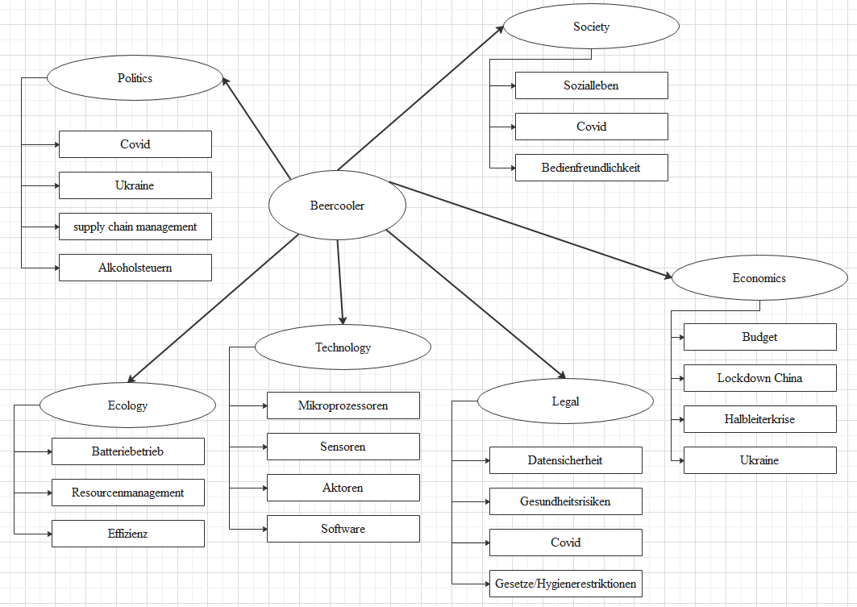
\includegraphics[width=\linewidth]{graphics/pestel.png}
\end{center}
\caption{Umfeld der Systemabgrenzung nach PESTEL}
\label{fig:pestel}
\end{figure}

\pagebreak

Das Eingriff System (Abbildung~\ref{fig:systemabgrenzung}) mit Umsystem hingegen 
vermittelt bereits ein deutlich klareres Bild.

\begin{figure}[h]
\begin{center}
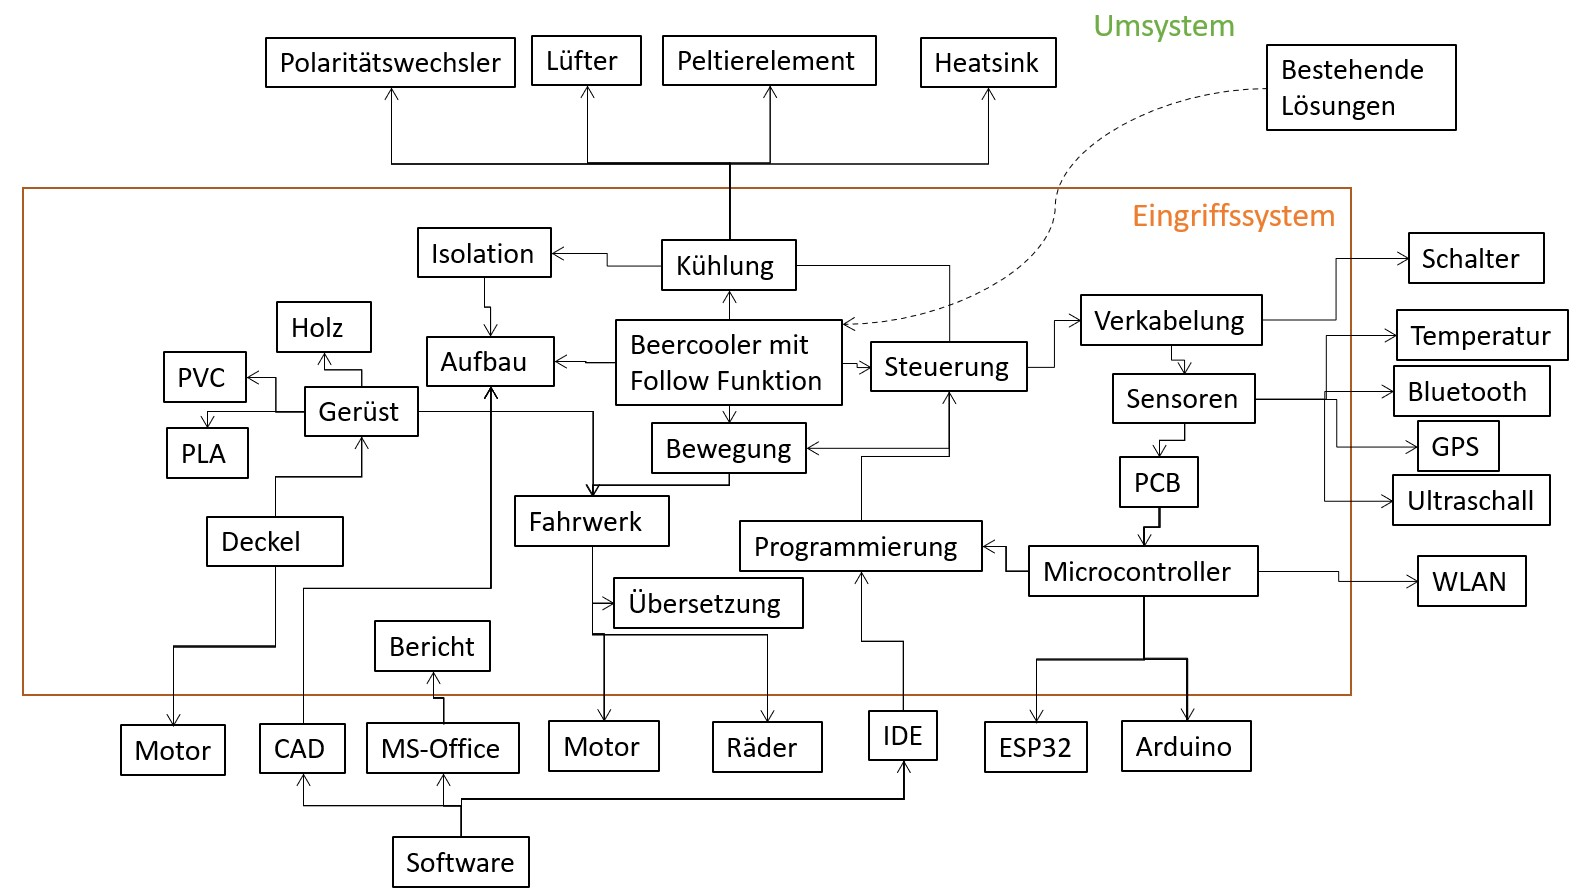
\includegraphics[width=\linewidth]{graphics/systemabgrenzung.jpg}
\end{center}
\caption{Umfeld der Systemabgrenzung nach PESTEL}
\label{fig:systemabgrenzung}
\end{figure}

\subsection{Zielkatalog}

Der Zielkatalog beschreibt unsere Anforderungen an das Projekt. Level 1 sind 
hierbei Ziele, die unbedingt erfüllt sein müssen, während Level 2 und 3 
Ausbaustufen darstellen, die weniger stark priorisiert werden. Zusammengefasst 
soll der Roboter also in der Lage sein, autonom einer Person zu folgen, 
mindestens ein Dutzend Bier zu beinhalten und diese über eine gewisse Zeit 
aktiv zu kühlen.

\textbf{Zielkatalog Level 1}



\textbf{Zielkatalog Level 2}



\textbf{Zielkatalog Level 3}


\section{Kapitel This}

\lipsum[9]

\subsection{Untertitel 1}

\lipsum[10]

\subsection{Untertitel 2}

\lipsum[11]

\subsubsection{Untertitel 3.~Grades}

Tabelle~\ref{tab:beispieltabelle} zeigt etwas. \lipsum[14-14]

\begin{table}
  \begin{center}
    \renewcommand{\arraystretch}{1.2}
    \begin{tabular}{l|S|S}\hline
      Medium & {Dichte $\rho$ in \SI{}{\kilogram\per\cubic\meter}} & 
               {Schallgeschwindigkeit $c$ in \SI{}{\meter\per\second}}\\
      \hline
		Luft \SI{0}{\degree C} trocken & 1.293 & 331 \\
		Wasserstoff \SI{0}{\degree C} & 0.090 & 1260 \\
		Wasser \SI{0}{\degree C} & 1000 & 1400 \\
		Holz & 600 & 4500 \\
		Stahl & 7700 & 5050 \\
		\hline
    \end{tabular}
  \end{center}
  \caption[Schallgeschwindigkeit in verschiedenen Medien]{Schallgeschwindigkeit in verschiedenen Medien gemäss \cite[S.~566]{hering_physik_2016}}
  \label{tab:beispieltabelle}
\end{table}

\lipsum[15-15]

\subsubsection{Untertitel 3.~Grades}

\lipsum[16-17]
\section{Kapitel That}

\lipsum[42]

\subsection{Code-Beispiel}

\lipsum[43]

\lstdefinestyle{custompython}{
  belowcaptionskip=1\baselineskip,
  breaklines=true,
  frame=L,
  xleftmargin=\parindent,
  numbers=left,
  language=Python,
  showstringspaces=false,
  basicstyle=\footnotesize\ttfamily,
  keywordstyle=\bfseries\color{green!40!black},
  commentstyle=\itshape\color{purple!40!black},
  identifierstyle=\color{blue},
  stringstyle=\color{orange},
}

\lstinputlisting[caption=Ein kurzes Codebeispiel in der Programmiersprache Python, style=custompython]{listings/python_example.py}

\section{Schlussbemerkungen}

\lipsum[28]


%%---BIBLIOGRAPHY------------------------------------------------------------------------
{\sloppypar
\printbibliography[heading=bibintoc, title=Quellenverzeichnis]
}

%%---APPENDIX----------------------------------------------------------------------------
\section*{Ehrlichkeitserklärung}
\addcontentsline{toc}{section}{Ehrlichkeitserklärung}

Hiermit erkläre ich, die vorliegende [Projektarbeit, Individualarbeit, Bachelorarbeit etc.] selbständig und nur unter Benutzung der angegebenen Quellen verfasst zu haben. Die wörtlich oder inhaltlich aus den aufgeführten Quellen entnommenen Stellen sind in der Arbeit als Zitat bzw. Paraphrase kenntlich gemacht. Diese [Studien-/Projektarbeit/Bachelor Thesis] ist noch nicht veröffentlicht worden. Sie ist somit weder anderen Interessierten zugänglich gemacht noch einer anderen Prüfungsbehörde vorgelegt worden.

\vspace*{4ex}

Windisch, tt. Monat 20jj

\vspace*{4ex}

{\renewcommand{\arraystretch}{2}
\begin{tabular}{@{}>{\bf}ll}
Name: & Pia Musterfrau\\
Unterschrift: & \\[6ex]
Name: & Michael Mustermann\\
Unterschrift: & \\
\end{tabular}
\begin{appendix} %Anhang
\section{Ein Anhang}

\lipsum[61-64]

\subsection{Aufgabenstellung im Originalwortlaut}

\lipsum[34]

\subsection{Gesamtübersicht}

\lipsum[35]

\subsection{Berechnungen / Resultate Umfrage}

\lipsum[36]

\subsection{Tests – Screenshots}

\lipsum[37]

%\includepdf[pages={1-2},nup=1x2,landscape=true,scale=0.85,offset=10 -40,pagecommand={\section{Eingefügtes Dokument; zwei Seiten auf einer}\label{app:Aufgabenstellung}\thispagestyle{myheadings}}]{appendix/aufgabenstellung.pdf} \newpage

%%Bei mehrseitigen Dokumenten die folgenden Seiten ohne Überschrift:
%\includepdf[pages={3-6},nup=1x2,landscape=true,scale=0.85,offset=10 -40,pagecommand={\thispagestyle{myheadings}}]{appendix/aufgabenstellung.pdf} \newpage

%\includepdf[pages={1},nup=1x1,landscape=true,scale=0.85,offset=10 -40,pagecommand={\section{Eingefügte PDF-Tabelle}\label{app:Timetable}\thispagestyle{myheadings}}]{appendix/timeline_example.pdf} \newpage

%%Bei mehrseitigen Dokumenten die folgenden Seiten ohne Überschrift:
%\includepdf[pages={2-5},nup=1x1,landscape=true,scale=0.85,offset=0 -20,pagecommand={\thispagestyle{myheadings}}]{appendix/timeline_example.pdf} \newpage

\end{appendix}


%%---NOTES for DEBUG---------------------------------------------------------------------
%\newpage
%\listoftodos[\section{Todo-Notes}]
%\clearpage

\end{document}